\documentclass[final,5p,12pt,twocolumn]{elsaarticle}

\usepackage{amssymb}
\usepackage{lipsum}
\usepackage{graphicx}
\usepackage{svg}
\newcommand{\kms}{km\,s$^{-1}$}
\newcommand{\msun}{$M_\odot}

\graphicspath{ {./images/} }


\begin{document}

\title{Comprehensive analysis of electronic noise and their noise spectra of zener diode}
\author{Vijay Panchal}
\author{Ved Rudani}
\address{Department of Physics, Electronics and Space Sciences, Gujarat University, Ahmedabad, India}

\begin{abstract}
    This is our semester project in which we studied noise from source \emph{zener diode} specifically BZX55C5V1. We looked for low frequency flicker noise, johnson noise and shot noise traces. In this project we used a lock-in amplifier specifically SR830 which is relatively accurate and low noise. We used the relative capability of SR830 that of minimum detection around 10nV/Hz signal. We made open source community with making python library \emph{pyinstro} for controlling and interfacing instruments like SR830. This program is made to be very flexible and highly extensible for use in every SCPI supported interface like GPIB, RS232, USB, LAN with capabilities like built-in file writer (.csv) and some CLI argument parsing.
\end{abstract}

\maketitle

\section{Introduction}\label{introduction}
Regulated power sources are extremely important in day to day lab work. Zener diodes and passive elements share an integral part of the overall circuit of regulated power supply.  When we are dealing with precision measurement and study we need the most precise power sources to work with but because of 'Noise' of components of zener diodes and passive elements it inherits noise internally. Since, this noise will be infested in precision work we are doing in the lab. It is better to study the known structure of noise in these devices to address methodic treatment to our data and circuits. With all this in mind we are doing noise measurement and studying the noise spectrum of the zener diode.



For this semester we had radical plans to try but it evolved into more mature or downgraded in a way. First tried as shot noise to generate a random number generator which could possibly be a true random generator with little transformations. Then we eyed the more on general idea of studying noise theoretically and doing analysis experimentally. Which is exactly what we are doing right now but change is that at start we are working with photodiode and now with zener diode. Thanks to Dr. U S Joshi sir who guided us to try different diodes against photodiode. In this report we are having the following parts in order. First we are studying theoretically components, then we will discuss methods and tools that we used included all instrumentation, data acquisition, data analysis etc., we will conclude with our results and discuss it. The foundational work in thermal noise was done by J B johnson in his paper \citep{johnson1928thermal}. 


\section{Theoritical compilation}\label{Theory}

We have a voltage regulator circuit from a zener diode which regulates voltages at specific voltage known as zener voltage $V_{z}$. The fluctuation from these regulated voltages is what we call noise. Since ideal regulators only give pure DC voltages at output, this fluctuation is completely unwanted and only be resultant of intrinsic noise of this regulator circuit . 


\begin{figure}[hbt!]
\centering{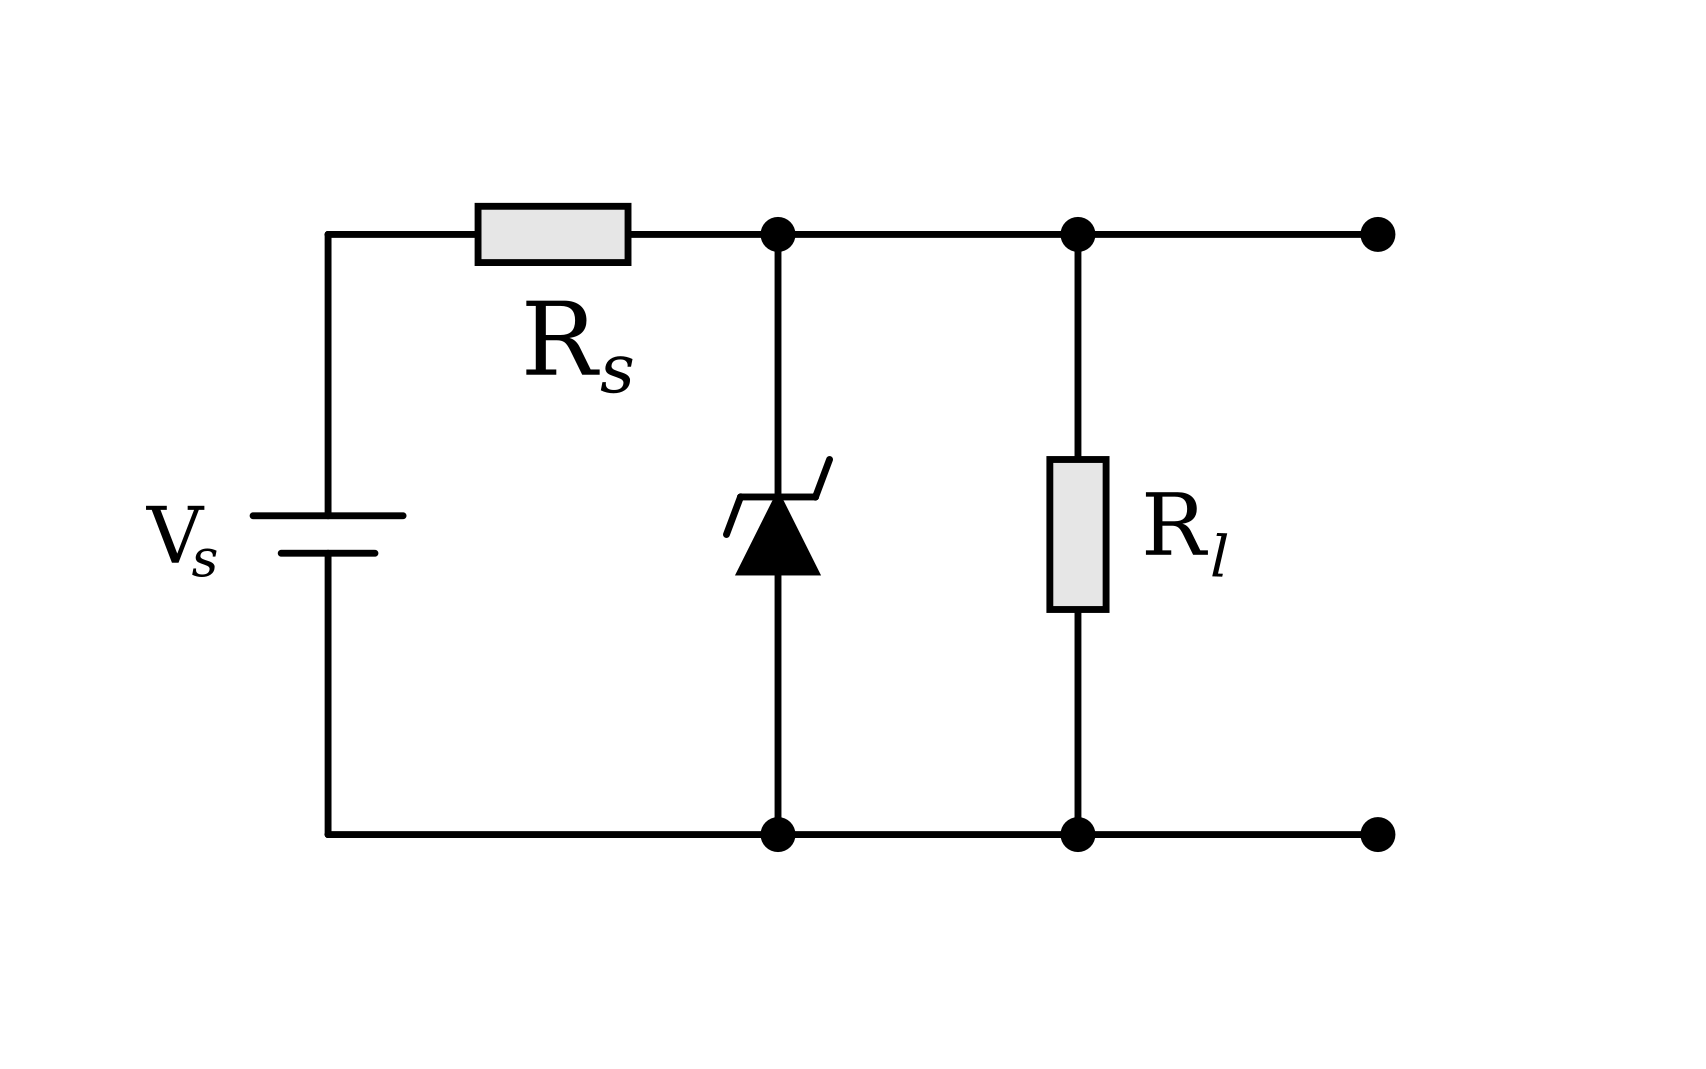
\includegraphics{circuit-20231005-2243.png}}
%% \centerline{\fbox{\vbox to 10pc{\vfill\hbox to 20pc{\hfill\Huge FPO\hfill}\vfill}}}
\caption{Response structure and positioning in the three zones.
FR, first responders.\label{fig1}}
\end{figure}

\begin{figure}[hbt!]
\centering{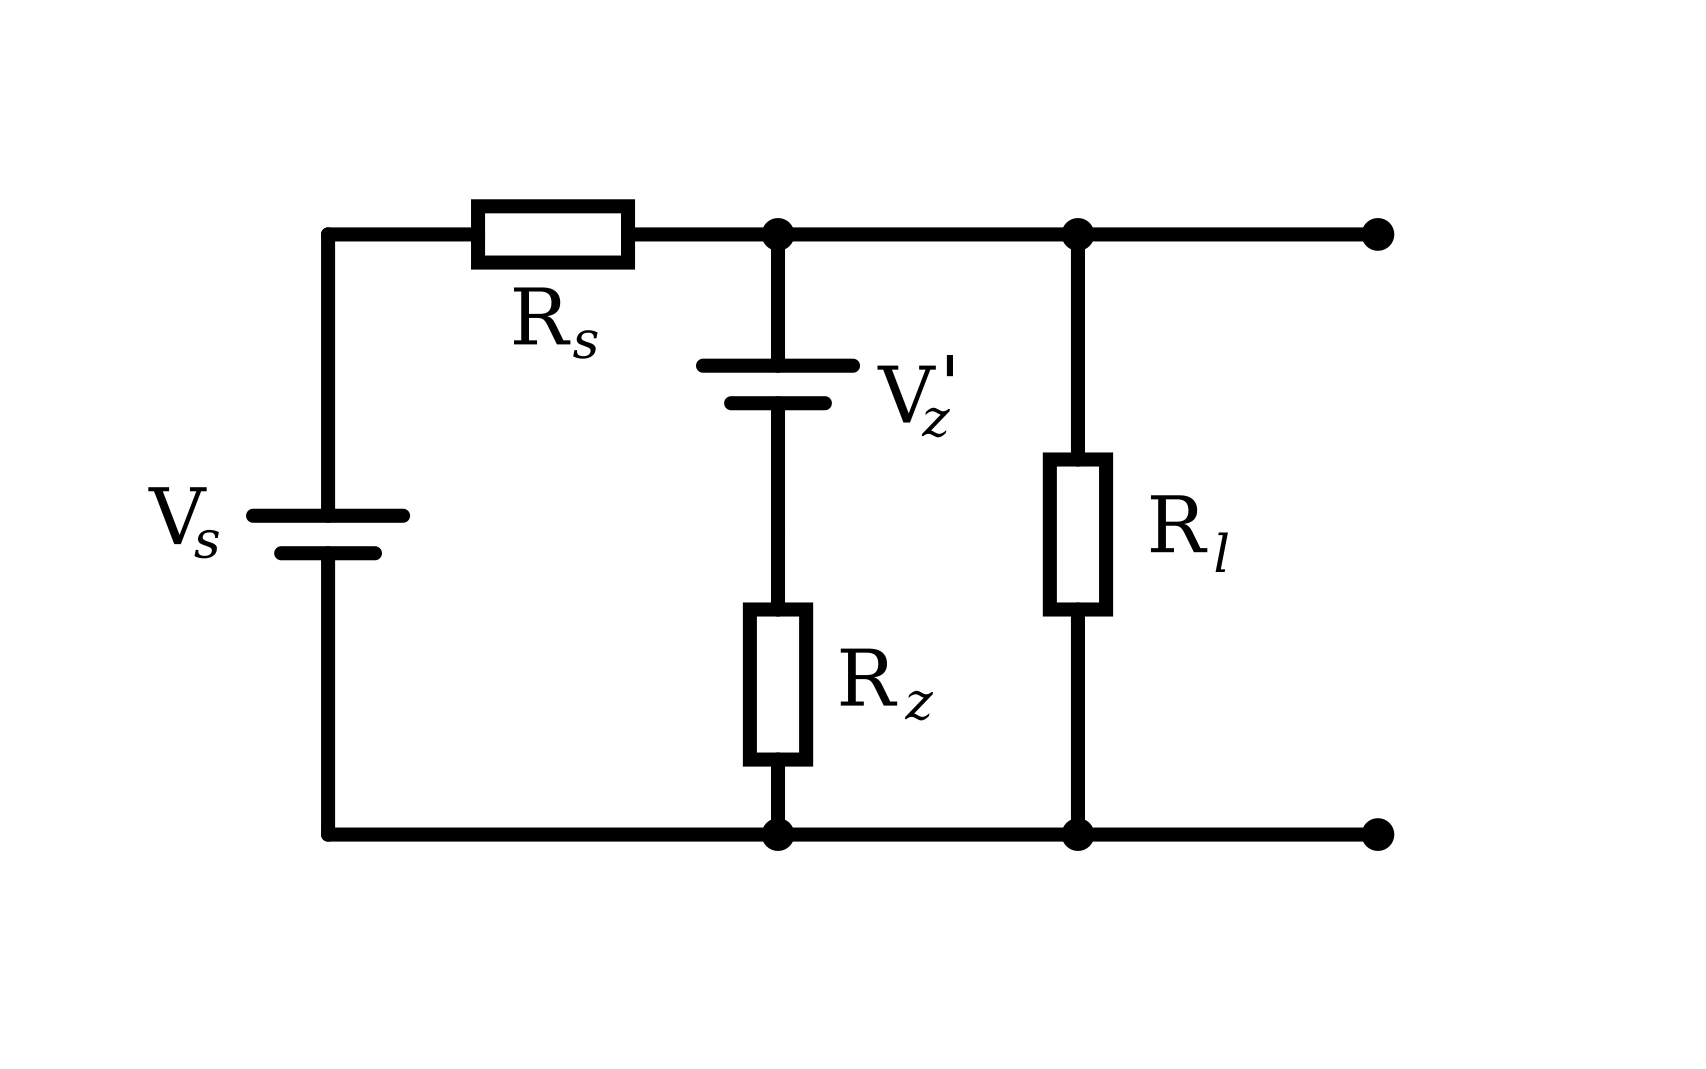
\includegraphics{circuit-20231005-2244.png}}
%% \centerline{\fbox{\vbox to 10pc{\vfill\hbox to 20pc{\hfill\Huge FPO\hfill}\vfill}}}
\caption{Response structure and positioning in the three zones.
FR, first responders.\label{fig2}}
\end{figure}

\begin{figure}[hbt!]
\centering{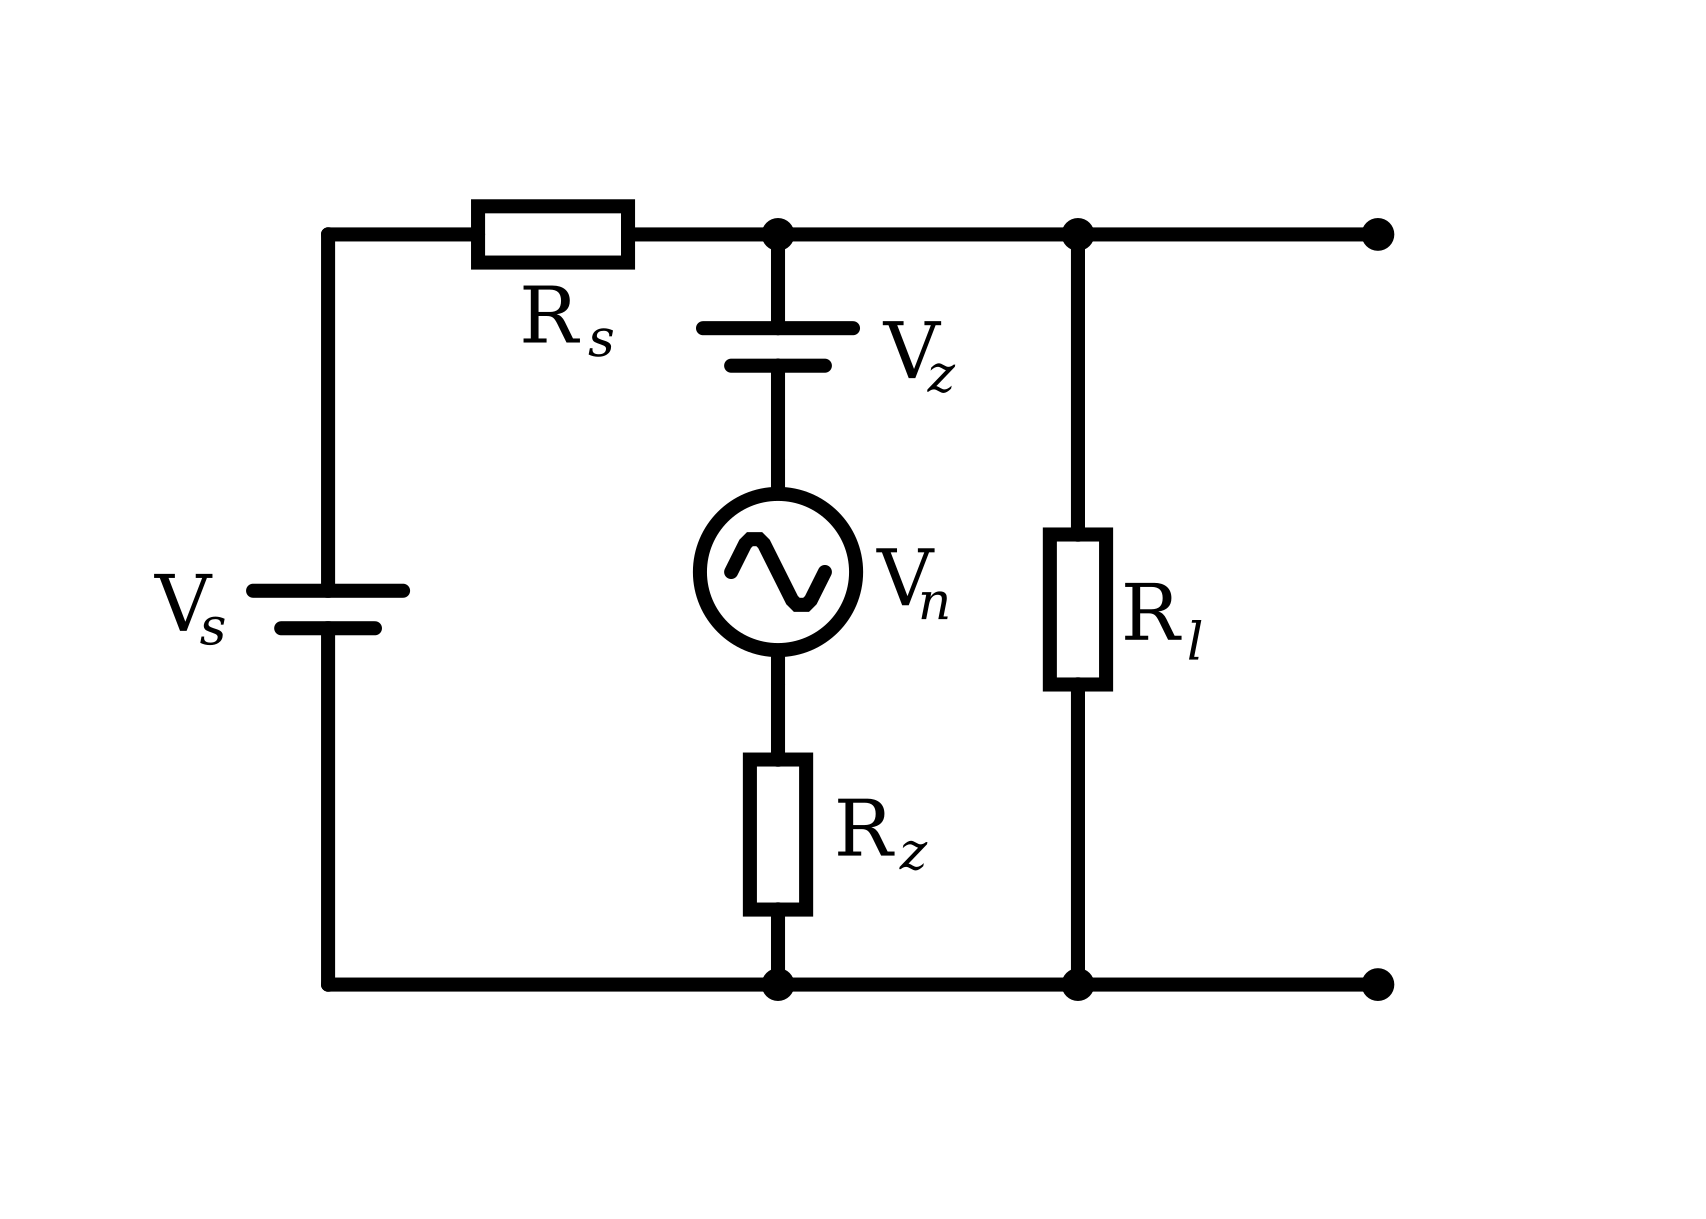
\includegraphics{circuit-20231005-2245.png}}
%% \centerline{\fbox{\vbox to 10pc{\vfill\hbox to 20pc{\hfill\Huge FPO\hfill}\vfill}}}
\caption{Response structure and positioning in the three zones.
FR, first responders.\label{fig3}}
\end{figure}


















\addcontentsline{toc}{section}{References}
\bibliographystyle{plain}
\bibliography{documentation}

\end{document}


